%%%%%%%%%%%%%%%%%%%%%%%%%%%%%%%%%%%%%%%%%
% Beamer Presentation
% LaTeX Template
% Version 1.0 (10/11/12)
%
% This template has been downloaded from:
% http://www.LaTeXTemplates.com
%
% License:
% CC BY-NC-SA 3.0 (http://creativecommons.org/licenses/by-nc-sa/3.0/)
%
%%%%%%%%%%%%%%%%%%%%%%%%%%%%%%%%%%%%%%%%%

%----------------------------------------------------------------------------------------
%	PACKAGES AND THEMES
%----------------------------------------------------------------------------------------

\documentclass{beamer}

\mode<presentation> {

% The Beamer class comes with a number of default slide themes
% which change the colors and layouts of slides. Below this is a list
% of all the themes, uncomment each in turn to see what they look like.

%\usetheme{default}
%\usetheme{AnnArbor}
%\usetheme{Antibes}
%\usetheme{Bergen}
%\usetheme{Berkeley}
%\usetheme{Berlin}
%\usetheme{Boadilla}
%\usetheme{CambridgeUS}
%\usetheme{Copenhagen}
%\usetheme{Darmstadt}
%\usetheme{Dresden}
%\usetheme{Frankfurt}
%\usetheme{Goettingen}
%\usetheme{Hannover}
%\usetheme{Ilmenau}
%\usetheme{JuanLesPins}
%\usetheme{Luebeck}
\usetheme{Madrid}
%\usetheme{Malmoe}
%\usetheme{Marburg}
%\usetheme{Montpellier}
%\usetheme{PaloAlto}
%\usetheme{Pittsburgh}
%\usetheme{Rochester}
%\usetheme{Singapore}
%\usetheme{Szeged}
%\usetheme{Warsaw}

% As well as themes, the Beamer class has a number of color themes
% for any slide theme. Uncomment each of these in turn to see how it
% changes the colors of your current slide theme.

%\usecolortheme{albatross}
%\usecolortheme{beaver}
%\usecolortheme{beetle}
%\usecolortheme{crane}
%\usecolortheme{dolphin}
%\usecolortheme{dove}
%\usecolortheme{fly}
%\usecolortheme{lily}
%\usecolortheme{orchid}
%\usecolortheme{rose}
%\usecolortheme{seagull}
%\usecolortheme{seahorse}
%\usecolortheme{whale}
%\usecolortheme{wolverine}

%\setbeamertemplate{footline} % To remove the footer line in all slides uncomment this line
%\setbeamertemplate{footline}[page number] % To replace the footer line in all slides with a simple slide count uncomment this line

%\setbeamertemplate{navigation symbols}{} % To remove the navigation symbols from the bottom of all slides uncomment this line
}

\usepackage{xeCJK}
\usepackage{fontspec}
\usepackage{graphicx} % Allows including images
\usepackage{booktabs} % Allows the use of \toprule, \midrule and \bottomrule in tables
\usepackage{subcaption}

%----------------------------------------------------------------------------------------
%	TITLE PAGE
%----------------------------------------------------------------------------------------

\title[General Relativity Raytracer]{基于相对论的天体引力模拟系统的研究} % The short title appears at the bottom of every slide, the full title is only on the title page

\author[李远恒]{李远恒\\ \vspace{3mm}\footnotesize 指导老师: 王庆娟}     % Your name
\institute[BITZH] % Your institution as it will appear on the bottom of every slide, may be shorthand to save space
{
北京理工大学珠海学院 \\ % Your institution for the title page
\medskip
\textit{liyh2077@gmail.com} % Your email address
}
\date{\today} % Date, can be changed to a custom date

\begin{document}

\begin{frame}
    \titlepage % Print the title page as the first slide
\end{frame}

% \begin{frame}
% \frametitle{Overview} % Table of contents slide, comment this block out to remove it
% \tableofcontents % Throughout your presentation, if you choose to use \section{} and \subsection{} commands, these will automatically be printed on this slide as an overview of your presentation
% \end{frame}

%----------------------------------------------------------------------------------------
%	PRESENTATION SLIDES
%----------------------------------------------------------------------------------------


\begin{frame}
    \frametitle{开发环境}
    \begin{description}
        \item[开发语言] C++
        \item[图形框架] QT
    \end{description}
\end{frame}

\begin{frame}
    \frametitle{黑洞简介}
    \begin{enumerate}
        \item 黑洞 \\ 黑洞是一片引力强大到连光都无法逃脱的区域
        \item 奇点 \\ 黑洞的中心是一个密度无穷大的奇点,奇点的时空也无限扭曲。黑洞奇点是造成时空扭曲并形成黑洞视界的根源;
        \item 事件视界 \\ 黑洞的视界是使黑洞称为黑洞的区域,视界以内的信息都无法向外传递,因为没有向外的路径存在。本文研究的限制在视界以外的区域(exterior);
        \item 引力透镜 \\ 黑洞本身是不能被看到的。但黑洞会扭曲周围的时空,通过观察周围物质的运动可以“看”到黑洞。黑洞就像一个圆形或者近似圆形透镜,会使远处传来的平行光产生偏折。
    \end{enumerate}

\end{frame}

\begin{frame}
    \frametitle{史瓦西黑洞的性质}
    史瓦西黑洞是最简单的黑洞,它拥有物理学中最重要的性质:
    \\~\\
    \begin{enumerate}
        \item 史瓦西黑洞是一个不旋转、不带电荷的黑洞;
        \item 史瓦西度规是一个球对称物体对时空造成的影响;
        \item 史瓦西时空是球对称的;
        \item 史瓦西度规不随时间$t$变化。
    \end{enumerate}
    ~\\
   史瓦西坐标为球坐标系$\left(ct,r,\theta,\phi\right)$
\end{frame}

\begin{frame}
    \frametitle{光线追踪}
    \begin{columns}[c] % The "c" option specifies centered vertical alignment while the "t" option is used for top vertical alignment

        \column{.45\textwidth} % Left column and width
        \textbf{传统光线追踪}
        \begin{figure}
            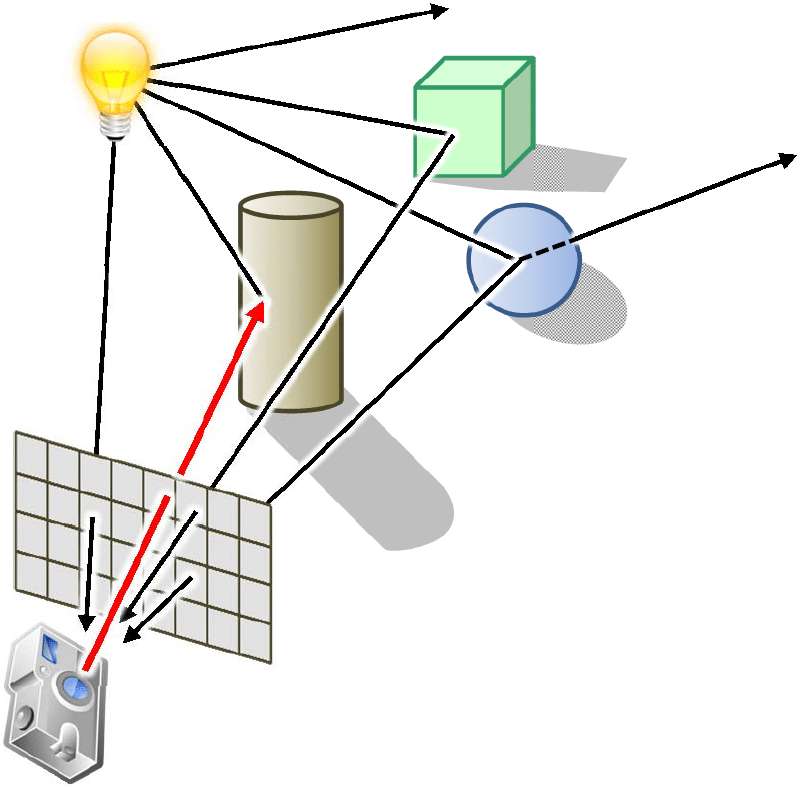
\includegraphics[width=0.8\linewidth]{Illustration-of-basic-ray-tracing.png}
        \end{figure}


        \column{.5\textwidth} % Right column and width
        \textbf{相对论引力模型光线传播}
        \begin{figure}
            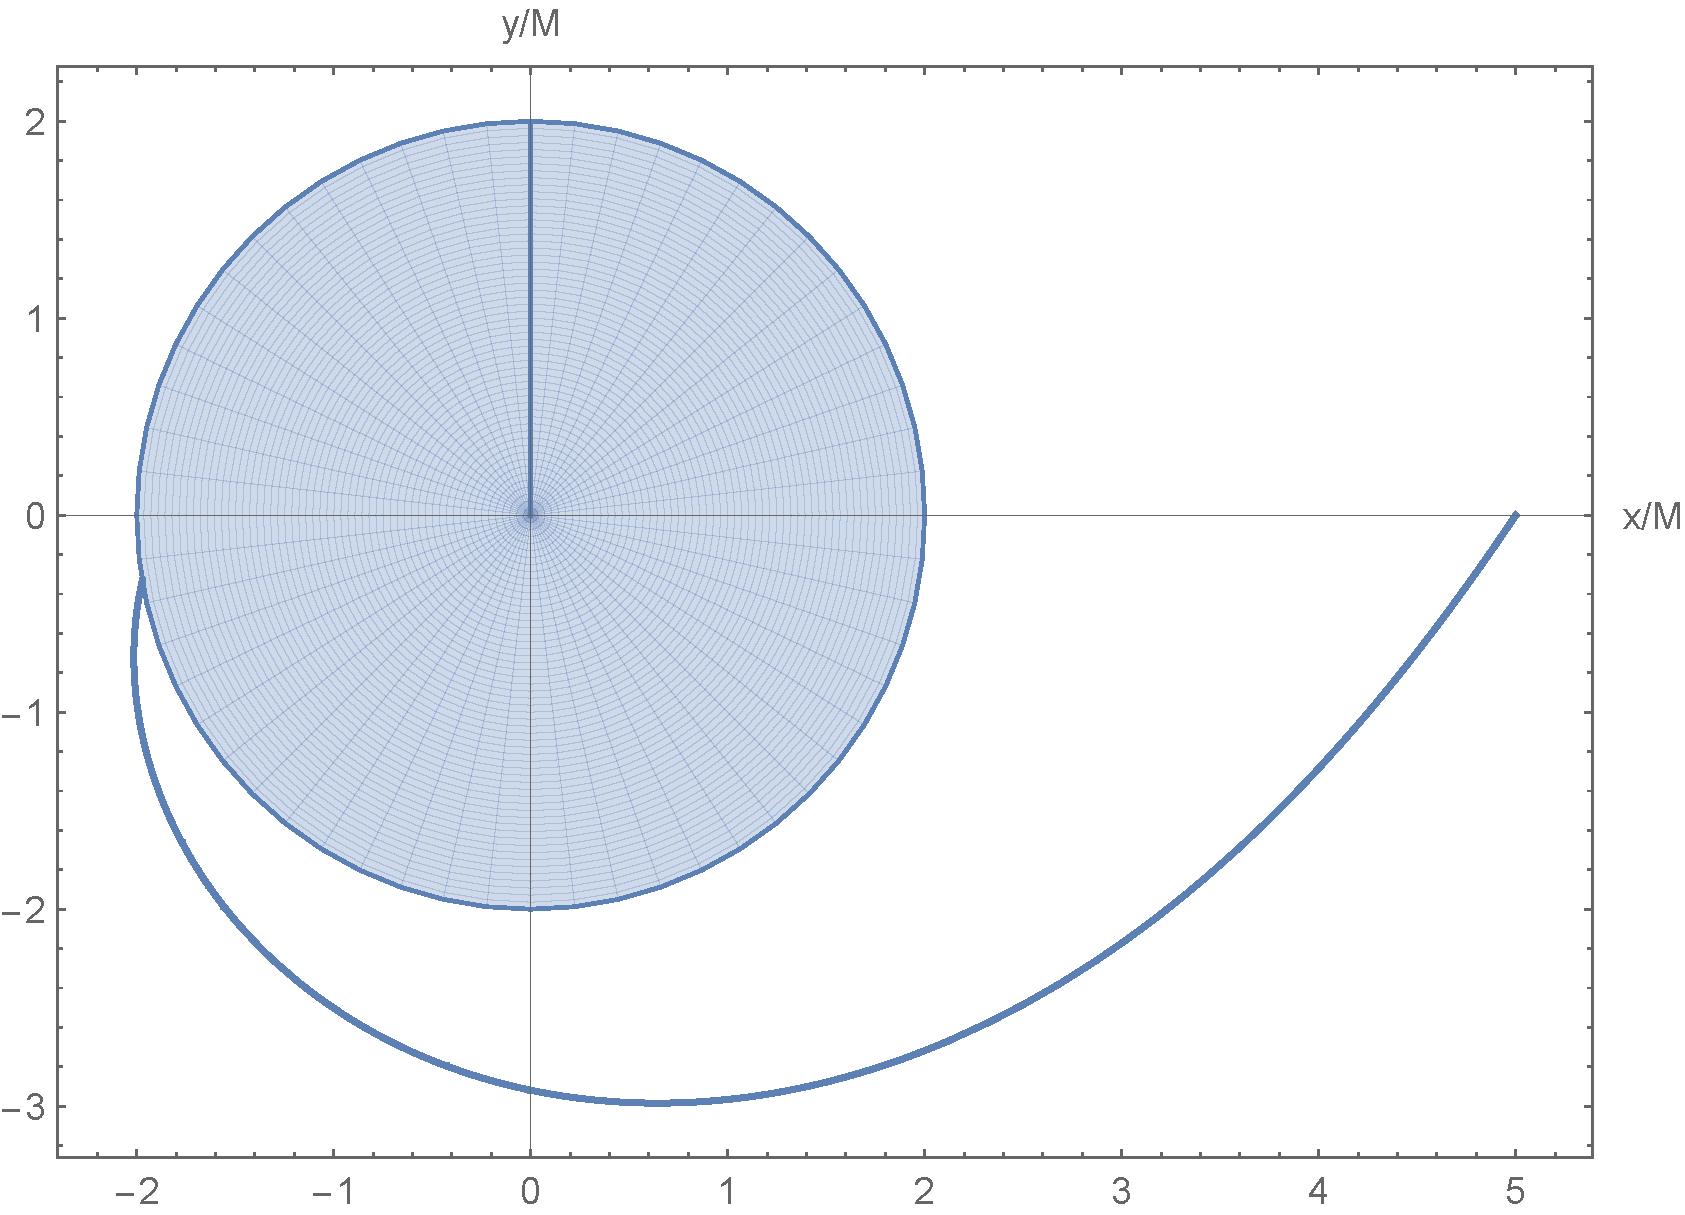
\includegraphics[width=0.8\linewidth]{ equatorial_plane_trace_2.pdf}
        \end{figure}

    \end{columns}
\end{frame}

%------------------------------------------------

\begin{frame}
    \frametitle{数学模型}
    \textbf{测地线方程}
    \begin{equation}
        ds^{2}=c^{2}\left(1-\frac{2MG}{c^{2}r}\right)dt^{2}-\left(1-\frac{2MG}{c^{2}r}\right)^{-1}dr^{2}-r^{2}d\theta^{2}-r^{2}\sin\theta^{2}d\phi^{2}
    \end{equation}
    \textbf{光线追踪公式}
    \begin{equation}
        \frac{d\phi}{dr}=\frac{1}{r^{2}\sqrt{\left(\frac{1}{b}\right)^{2}-\frac{1}{r^{2}}\left(1-\frac{2GM}{c^{2}r}\right)}}\label{eq:geodesic}
    \end{equation}
    \textbf{撞击参数}
    \begin{equation}
        b=\frac{r\sin\theta}{\sqrt{1-\frac{r_{s}}{r}}}
    \end{equation}
\end{frame}

%------------------------------------------------

\begin{frame}
    \frametitle{模型的边界条件}
    \begin{columns}[c] % The "c" option specifies centered vertical alignment while the "t" option is used for top vertical alignment

        \column{.45\textwidth} % Left column and width
        \textbf{设定}
        \begin{description}
            \item[坐标系] 笛卡尔坐标系
            \item[单位制] $\frac{GM}{c^2}=M$
            \item[黑洞] 置于世界坐标中心
        \end{description}


        \column{.5\textwidth} % Right column and width
        \textbf{输入}
        \begin{description}
            \item[吸积盘] 内径、外径与材质
            \item[天空盒] 六面材质
            \item[相机] 坐标,面对方向
        \end{description}

    \end{columns}
\end{frame}

\begin{frame}
    \frametitle{光线追踪流程图}
    \begin{figure}[H]
        \centering
        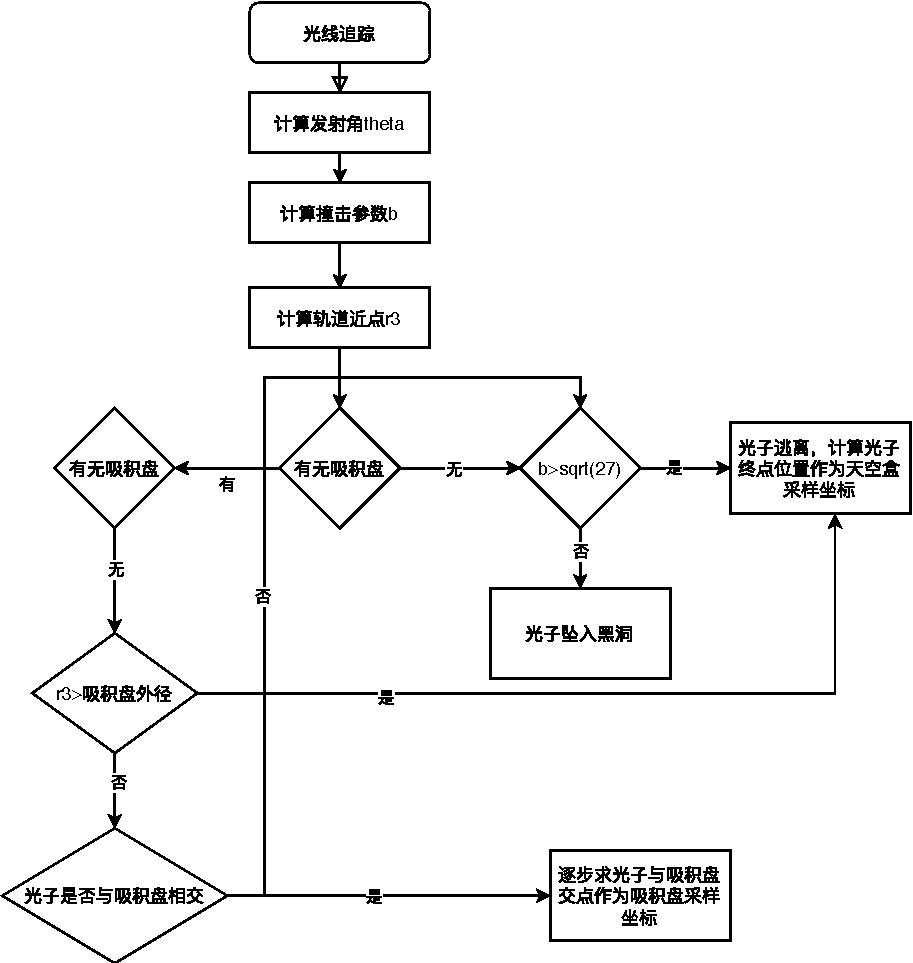
\includegraphics[scale=0.45]{images/flowchart.pdf}
    \end{figure}
\end{frame}



\begin{frame}
    \frametitle{系统优点-速度}
    本设计渲染性能比其他渲染器如starless高一个数量级,测试设定如下:
    \begin{itemize}
        \item 相机位置$(0, 1, 10)$;
        \item 分辨率$1024\times1024$;
        \item 渲染线程数16。
    \end{itemize}
    \begin{figure}[H]
        \centering
        \begin{subfigure}{.45\textwidth}
            \centering
            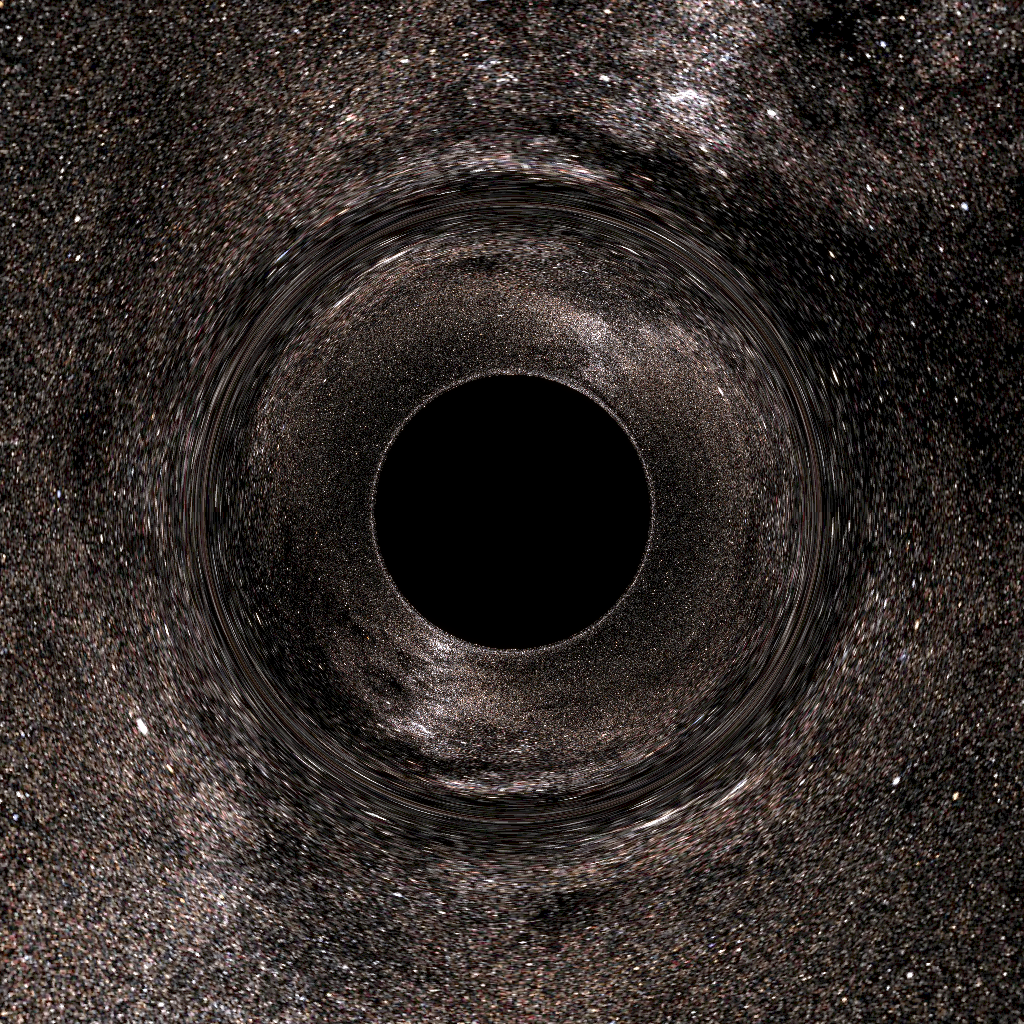
\includegraphics[width=.8\linewidth]{images/starless_test.png}
            \caption{starless渲染的图片-41秒}
            \label{fig:starless_test}
        \end{subfigure}%
        \begin{subfigure}{.45\textwidth}
            \centering
            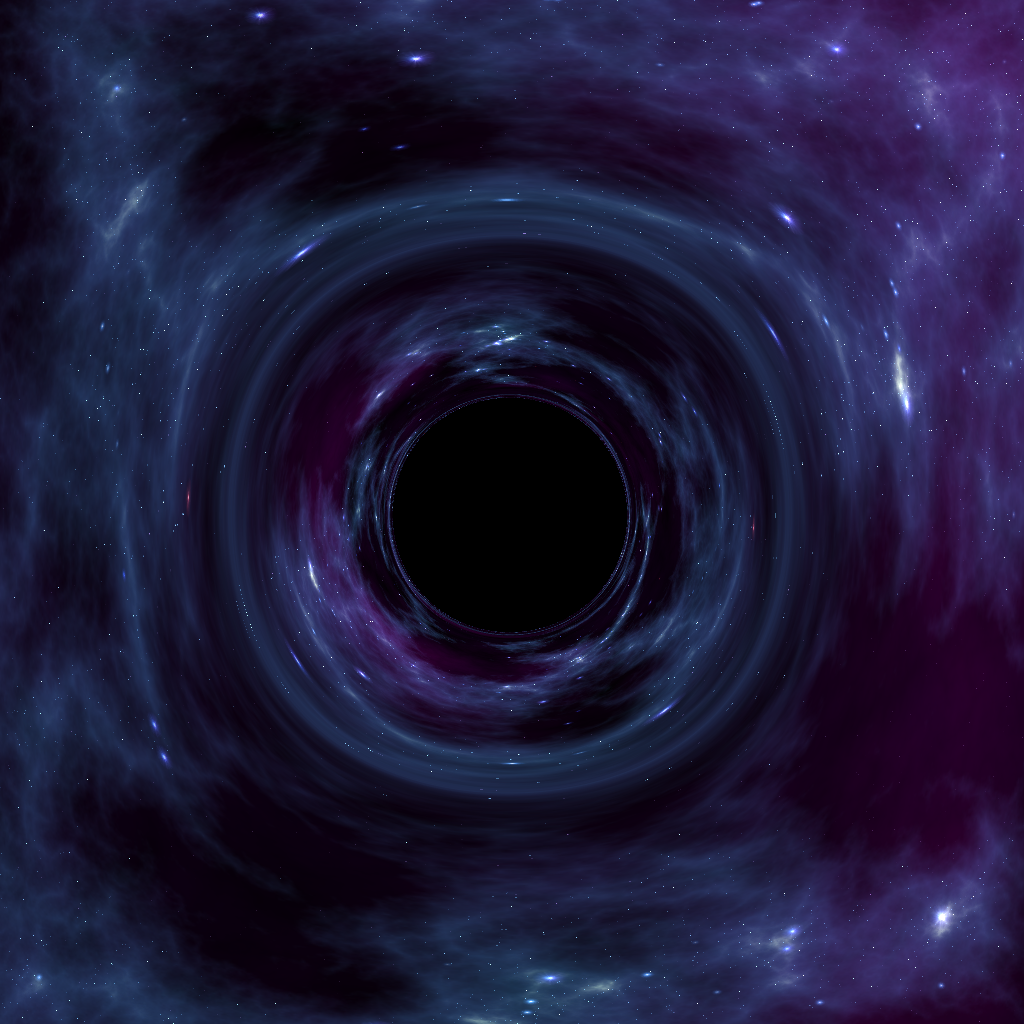
\includegraphics[width=.8\linewidth]{images/blackness_test.png}
            \caption{本设计渲染的图片-1.2秒}
            \label{fig:blackness_test}
        \end{subfigure}
    \end{figure}

\end{frame}

\begin{frame}
    \frametitle{系统优点-精度}
    生成的图片可以放大万倍看到光线围绕黑洞旋转两圈半的次级像
    \begin{figure}[H]
        \centering
        \begin{subfigure}{.24\textwidth}
            \centering
            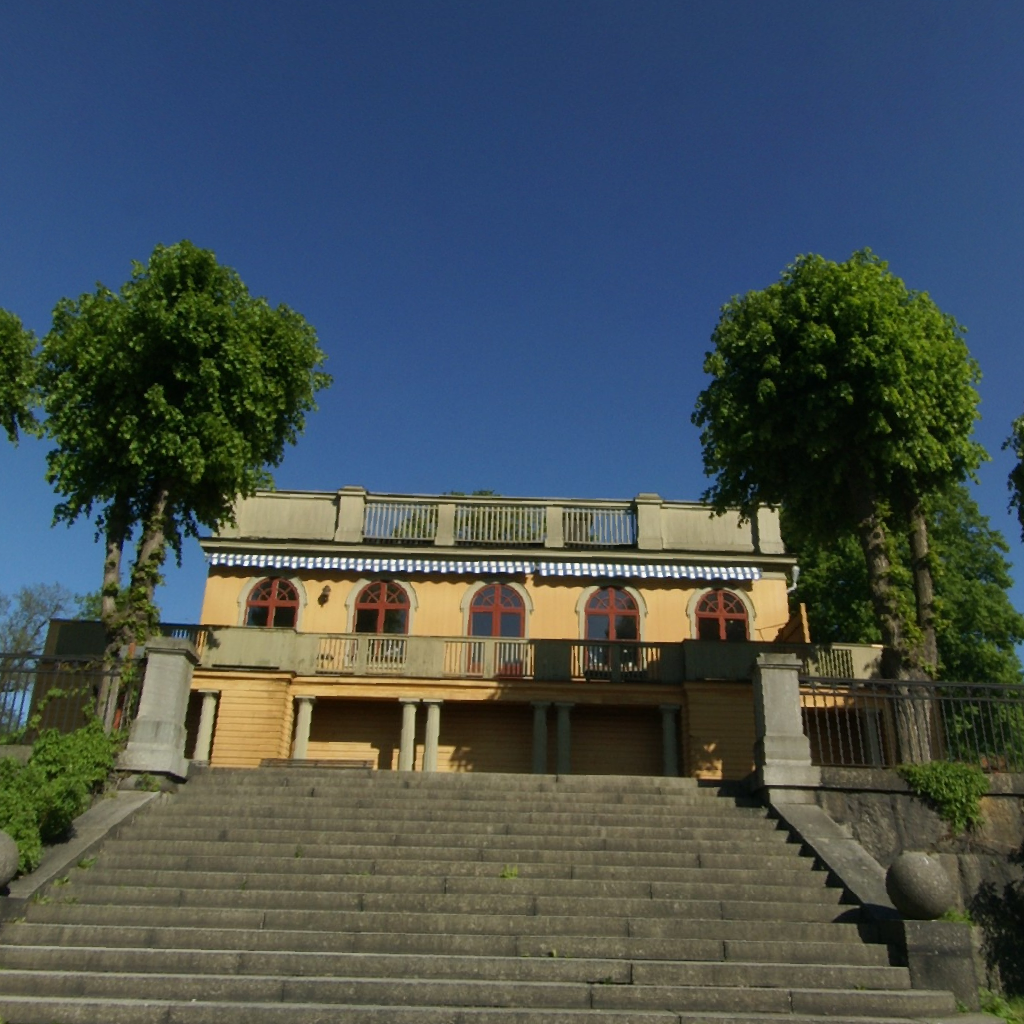
\includegraphics[width=.8\linewidth]{images/building.png}
            \caption{原始}
            \label{fig:starless_test}
        \end{subfigure}%
        \begin{subfigure}{.24\textwidth}
            \centering
            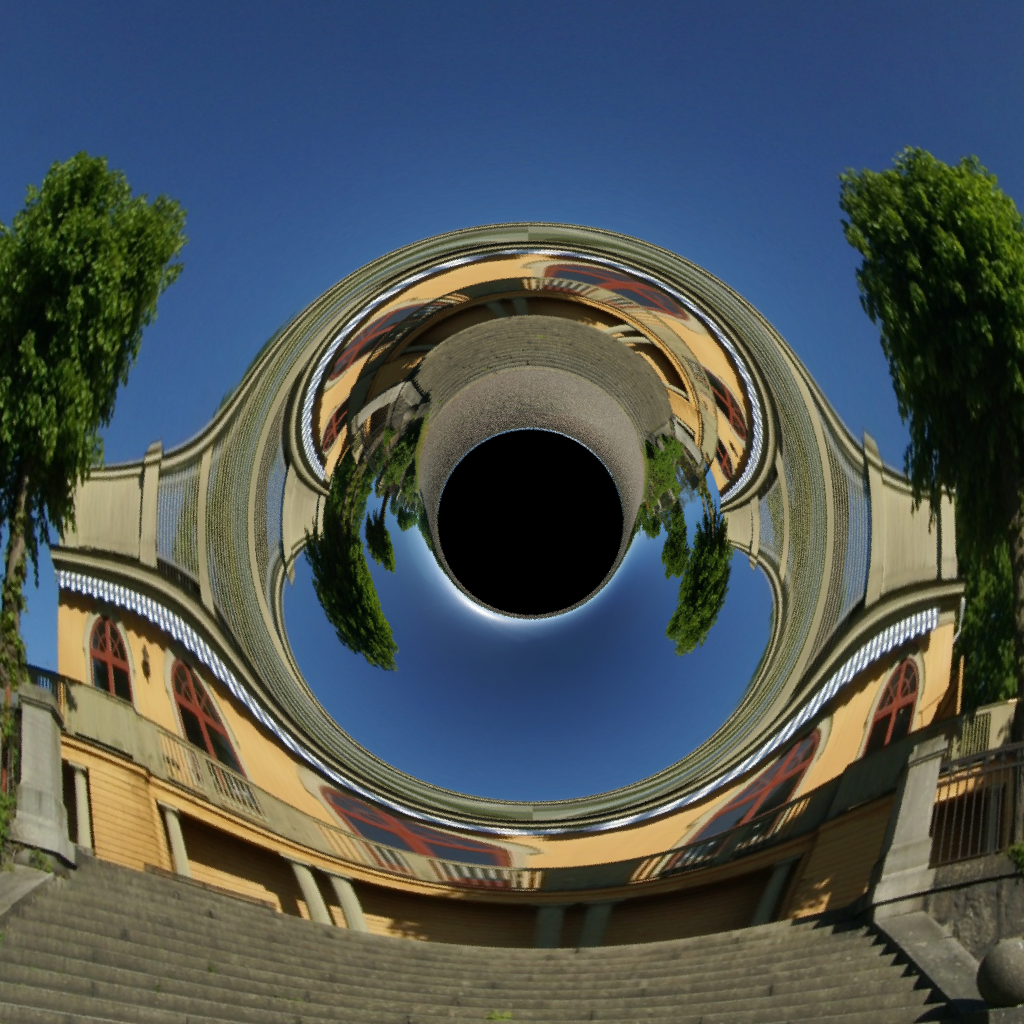
\includegraphics[width=.8\linewidth]{images/building_distort.png}
            \caption{1倍}
            \label{fig:blackness_test}
        \end{subfigure}
        \begin{subfigure}{.24\textwidth}
            \centering
            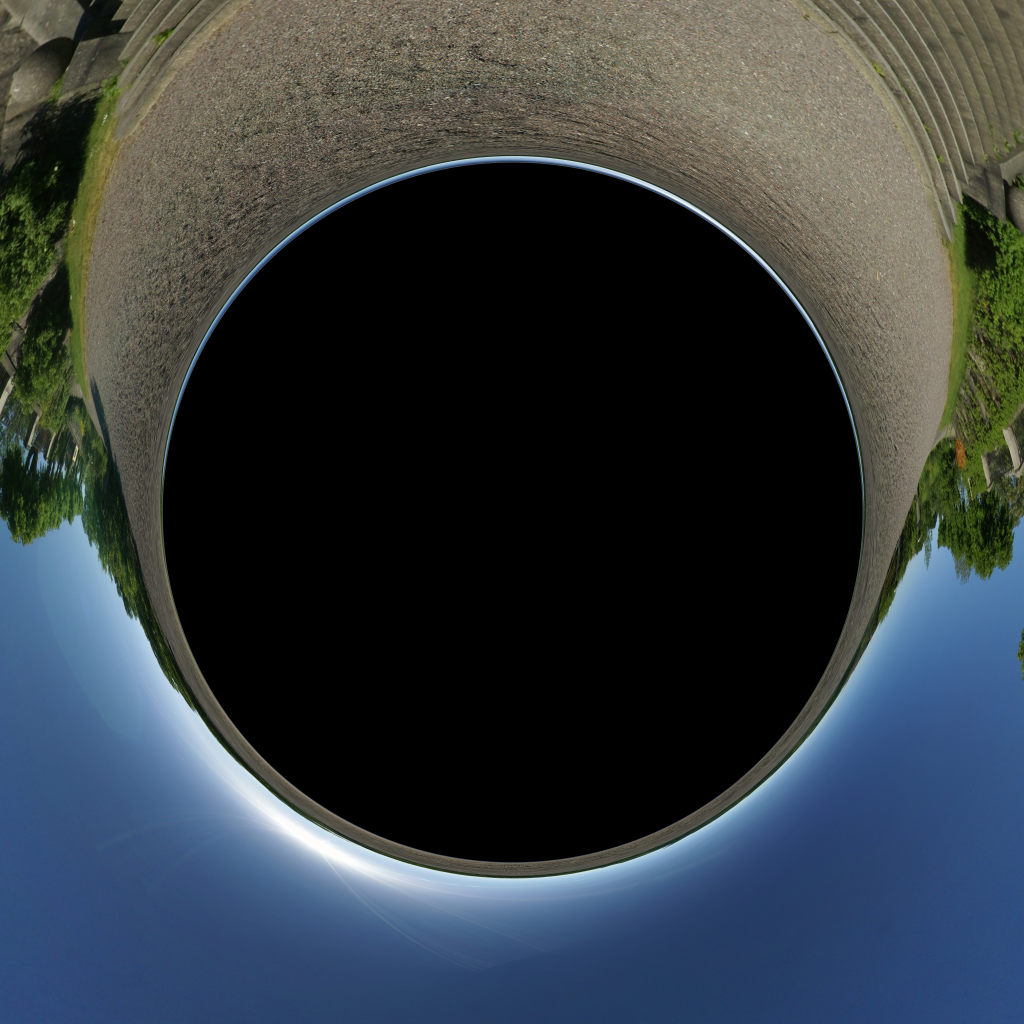
\includegraphics[width=.8\linewidth]{images/zoomin_6x.png}
            \caption{6倍}
            \label{fig:blackness_test}
        \end{subfigure}
        \begin{subfigure}{.24\textwidth}
            \centering
            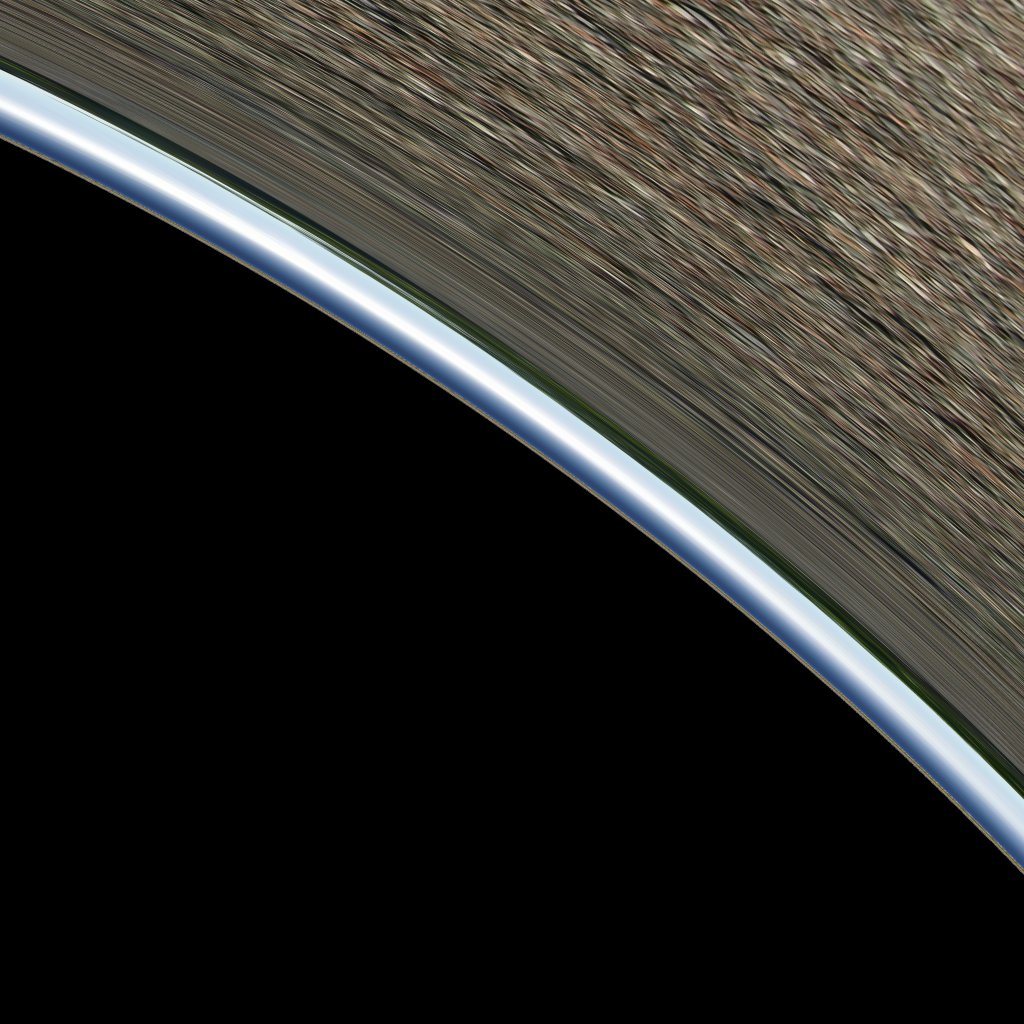
\includegraphics[width=.8\linewidth]{images/zoomin_60x.png}
            \caption{60倍}
            \label{fig:blackness_test}
        \end{subfigure}

        \centering
        \begin{subfigure}{.33\textwidth}
            \centering
            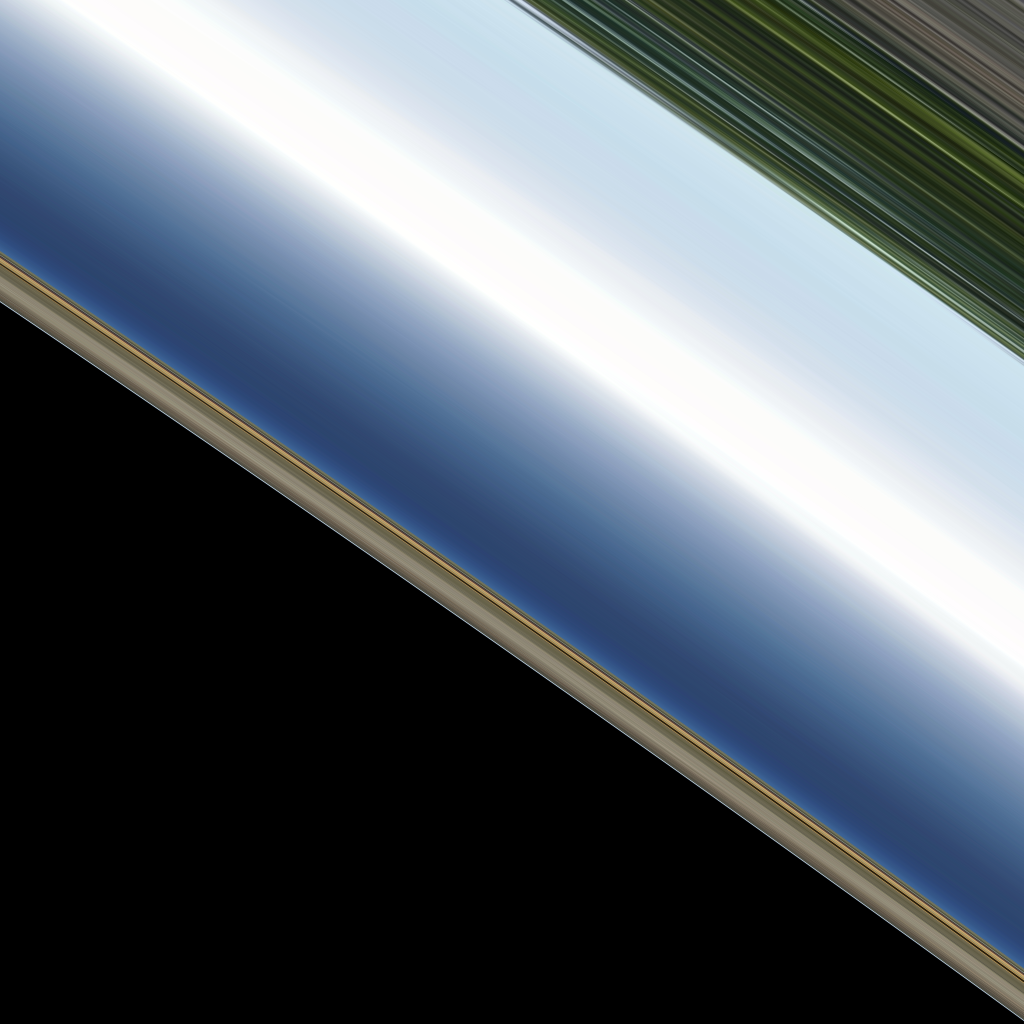
\includegraphics[width=.8\linewidth]{images/zoomin_600x.png}
            \caption{600倍}
            \label{fig:starless_test}
        \end{subfigure}%
        \begin{subfigure}{.33\textwidth}
            \centering
            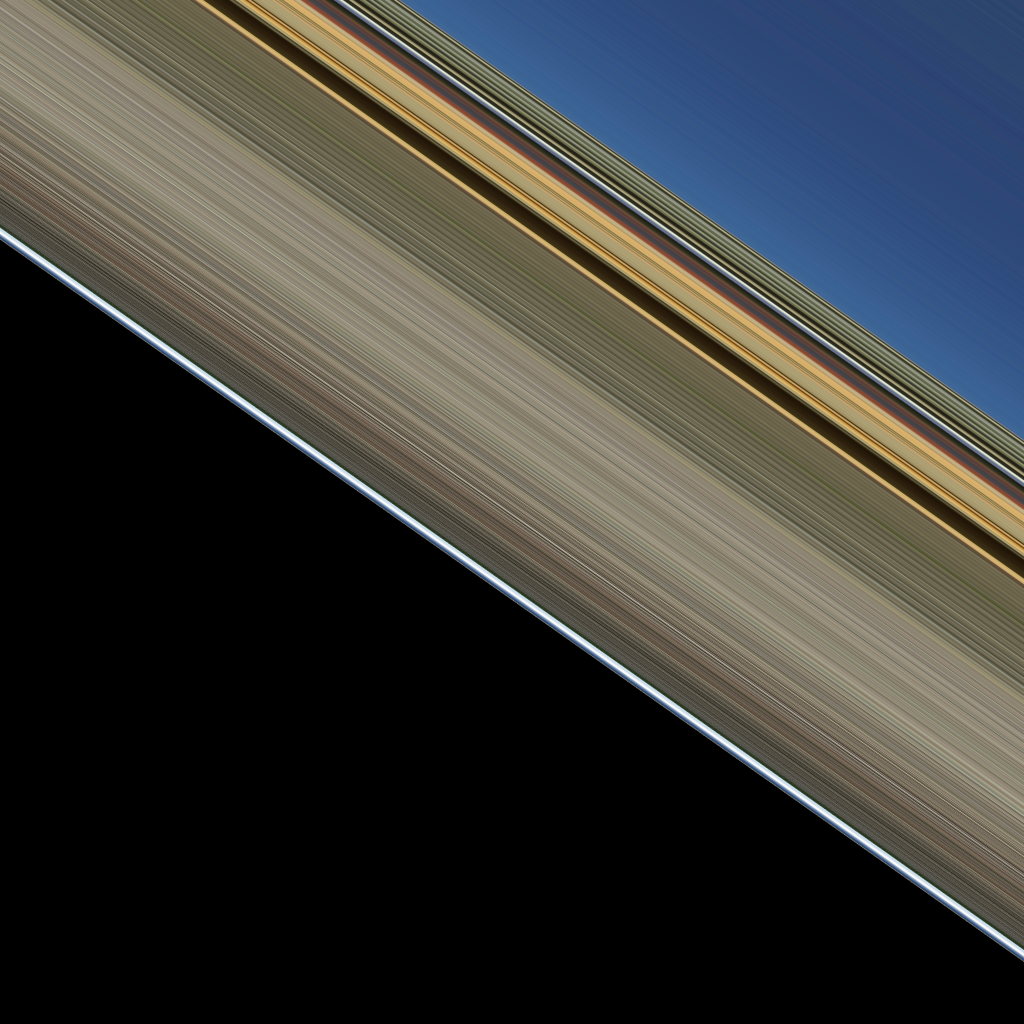
\includegraphics[width=.8\linewidth]{images/zoomin_6000x.png}
            \caption{6000倍}
            \label{fig:blackness_test}
        \end{subfigure}
        \begin{subfigure}{.33\textwidth}
            \centering
            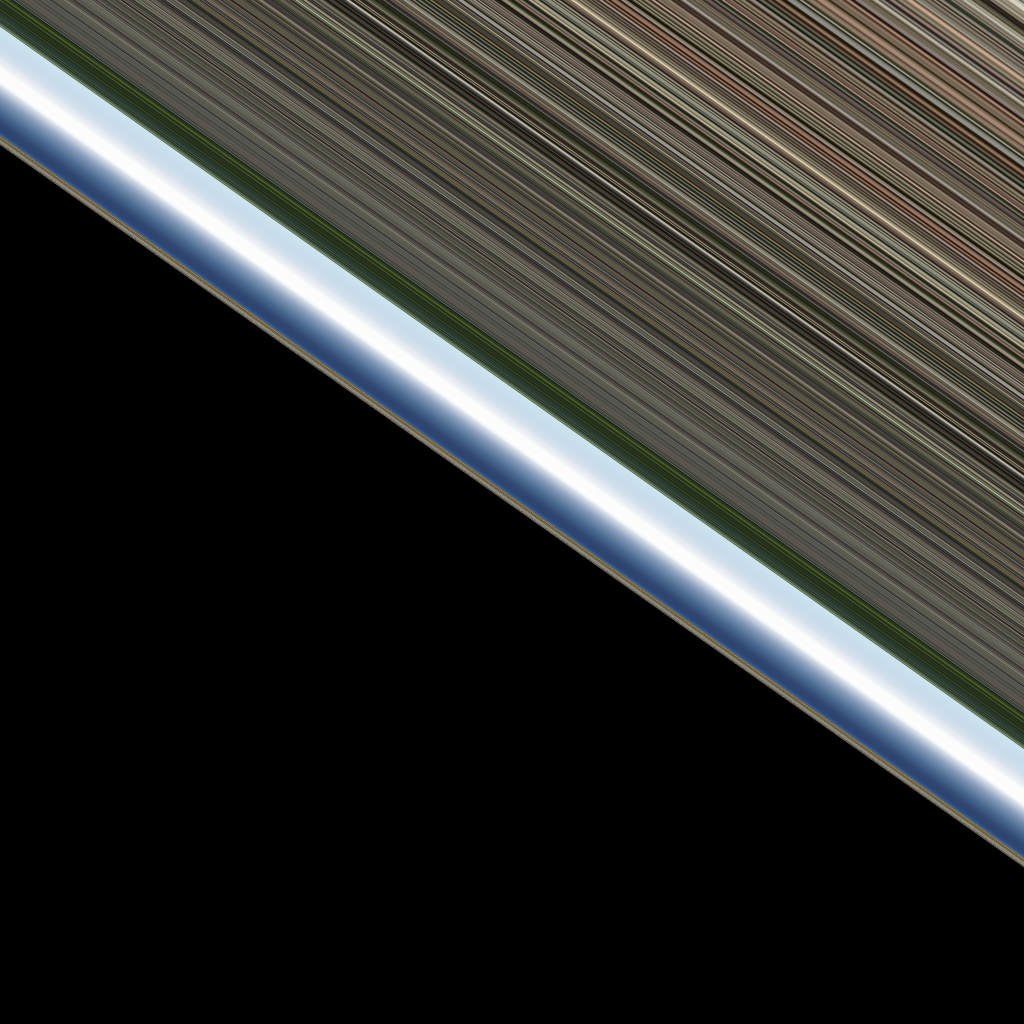
\includegraphics[width=.8\linewidth]{images/zoomin_60000x.png}
            \caption{60000倍}
            \label{fig:blackness_test}
        \end{subfigure}
    \end{figure}

\end{frame}


\begin{frame}
    \frametitle{改进方向}
    \begin{enumerate}
        \item 更快的积分方法
        \item 吸积盘支持alpha通道
        \item 支持旋转的中心天体
    \end{enumerate}

\end{frame}

%------------------------------------------------

\begin{frame}
    \frametitle{References}
    \setlength{\parskip}{0.5em}
    \fontsize{6pt}{7.2}\selectfont
    [1]Black hole.//Wikipedia. [S.l. : s.n.], 2020.

    [2]Gillessen S, Eisenhauer F, Trippe S, et al. Monitoring stellar orbits around the Massive Black Hole inthe Galactic Center[J]. The Astrophysical Journal, 2009, 692(2):1075­1109. arXiv:0810.4674.

    [3]Garner R. NASA Visualization Shows a Black Hole’s Warped World: NASA[EB/OL]. (2019­09­25)[2020­05­05].http://www.nasa.gov/feature/goddard/2019/nasa­visualization­shows­a­black­hole­s­warped­world.

    [4]Riazuelo A. Too Close to a Black Hole[EB/OL]. 2010[2020­04­02].https://apod.nasa.gov/apod/ap101207.html.

    [5]Raytracing a Black Hole[EB/OL]. [2020­05­05].http://rantonels.github.io/starless/.

    [6]Light cone.//Wikipedia. [S.l. : s.n.], 2020.[8]Mueller T, Grave F. Catalogue of Spacetimes[J]. ArXiv:0904.4184 [gr­qc], 2010. arXiv:0904.4184.

    [7]Riazuelo A. Seeing relativity – I. Ray tracing in a Schwarzschild metric to explore the maximal analyticextension of the metric and making a proper rendering of the stars[J]. ArXiv:1511.06025 [gr­qc], 2018.arXiv:1511.06025.

    [8]Rotation matrix.//Wikipedia. [S.l. : s.n.], 2020.

    [9]Ordinary Differential Equation Solvers ODE23 and ODE45: Cleve’s Corner: Cleve Moler on Math­ematics and Computing[EB/OL]. [2020­05­03].https://blogs.mathworks.com/cleve/2014/05/26/ordinary­differential­equation­solvers­ode23­and­ode45/.

    [10]Mathews J H, Fink K D. Numerical methods using MATLAB[M]. 4th ed. Upper Saddle River, N.J:Pearson, 2004. 680 pp.

    [11]James O, von Tunzelmann E, Franklin P, et al. Gravitational Lensing by Spinning Black Holes inAstrophysics, and in the Movie Interstellar[J]. Classical and Quantum Gravity, 2015, 32(6):065001. arXiv:1502.03808.

    [12]Nvidia. NVIDIA­Turing­Architecture­Whitepaper.pdf[EB/OL]. [2020­04­21].https://www.nvidia.com/content/dam/en­zz/Solutions/design­visualization/technologies/turing­architecture/NVIDIA­Turing­Architecture­Whitepaper.pdf.

\end{frame}


%------------------------------------------------

\begin{frame}
    \huge{\centerline{感谢各位评委老师的批评和指正}}
    \vspace{8mm}
    \Large{\centerline{感谢国家天文台许优华博士}}
    \Large{\centerline{对本论文的帮助和支持}}
\end{frame}

%----------------------------------------------------------------------------------------

\end{document}